% \documentclass[rmp,aps,floatfix,authordate1-4,preprint]{revtex4}
% \documentclass[prb,aps,floatfix,authordate1-4,preprint]{revtex4}

\documentclass[pre,aps,floatfix,authordate1-4,twocolumn]{revtex4-1}
%\documentclass[pre,aps,floatfix,authordate1-4]{revtex4-1}

%\documentclass[aps,prl,preprint,superscriptaddress]{revtex4}



%\documentclass[aps,prl,preprint,groupedaddress]{revtex4}

\usepackage{rotating} 
\usepackage{times}
\usepackage{graphicx}
\usepackage{setspace}
\usepackage{amsmath}
\usepackage{caption}
\usepackage{subcaption}
\usepackage{epstopdf}
%\usepackage{array}
%\usepackage{arydshln}
%\usepackage[sort&compress]{natbib}
%\bibpunct{(}{)}{,}{n}{}{}
%\renewcommand{\bibnumfmt}[1]{#1.}
\usepackage[obeyFinal]{easy-todo}

\usepackage[normalem]{ulem}

\begin{document}
%\singlespacing

\title{The electrometer concept and binding of cations to phospholipid bilayers}

\author{Andrea Catte}
\thanks{The authors are listed in alphaphetical order.}
\thanks{The author list is not completed.}
\thanks{University of East Anglia, Norwich, United Kingdom}
\author{Mykhailo Girych}
\thanks{Helsinki Biophysics and Biomembrane Group, Department of Biomedical Engineering and Computational Science, Aalto University, Espoo, Finland}
\author{Matti Javanainen}
\thanks{Tampere University of Technology, Tampere, Finland}
\author{Markus S. Miettinen}
\thanks{Fachbereich Physik, Freie Universit\"at Berlin, Berlin, Germany}
\author{Luca Monticelli}
\thanks{Institut de Biologie et Chimie des Prot{\'e}ines (IBCP), CNRS UMR 5086, Lyon, France}
%\setcounter{page}{1}
\author{Jukka M{\"a}{\"a}tt{\"a}}
\thanks{Aalto University, Espoo, Finland}
\author{Vasily S. Oganesyan}
\thanks{University of East Anglia, Norwich, United Kingdom}
\author{O. H. Samuli Ollila} 
\thanks{{\bf Author to whom correspondence may be addressed. E-mail: samuli.ollila@aalto.fi.}}
\thanks{Helsinki Biophysics and Biomembrane Group, Department of Biomedical Engineering and Computational Science, Aalto University, Espoo, Finland}
%\footnote{Author to whom 
%correspondence may be addressed. E-mail: samuli.ollila@aalto.fi.\\
%}
%\affiliation{
%  Helsinki Biophysics and Biomembrane Group,
%Department of Biomedical Engineering and Computational Science, Aalto University, Espoo, Finland
%}



\begin{abstract}
%We compare the order parameters predicted for the hydrocarbon segments in lipid bilayer headgroup region
%by the Berger molecular dynamics simulation model to those measured by Nuclear Magnetic Resonance (NMR) experiments.
%We first show results for a fully hydrated POPC bilayer, and then focus on changes of the order parameters as
%a function of hydration level, NaCl and CaCl$_2$ concentrations, and cholesterol content. The experimental headgroup order 
%parameters are never reproduced.
%This indicates that under all of these conditions the used model is unable to correctly reproduce the headgroup structure. 
%Consequently, many of the conclusions drawn over the years from this model might be erroneous.
%This manuscript has not been submitted to any journal, instead its contents are discussed at 
%nmrlipids.blogspot.fi.
Despite of vast amount of experimental and theoretical studies, the binding affinity of cations, especially the biologically relevant Na$^+$ and Ca$^{2+}$ ions,
into a phosholipid bilayer is not agreed on in the literature. Here we directly compare the measured choline headgroup order parameters
to the simulations with different models in the presence of different cations. We conclude that the simplest explanation
for the experimental and theoretical observations is that at mM concentrations the Na$^+$ ions do not  \sout{penetrate into} bind to \todo{Markus: 'penetrate into' gives the impression they go really deep, that is, even in the tails. On the other hand, 'bind to' could mean that they are bound just to the headgroup region. Should we maybe say precisely until where do they penetrate?}
phosphatidylcholine lipid bilayers, in contrast to Ca$^{2+}$. Further, the binding affinity of Na$^+$ is overestimated in almost all molecular dynamics simulation models.
However, the electrometer concept (connecting the choline order parameter changes to the amount of penetrating charge) is valid also in simulations.

{\it This work has been, and continues to be, progressed and discussed through the blog: nmrlipids.blogspot.fi.
Everyone is invited to join the discussion and make contributions through the blog. The manuscript will be
eventually submitted to an appropriate scientific journal. Everyone who has contributed to the work through the
blog will be offered coauthorship. For more details see: nmrlipids.blogspot.fi.}
\end{abstract}


\maketitle


~\vspace{0.3cm}\\
{\it \bf} 

\section{Introduction}

The cation interactions with phospholipid membranes occur in a large amount
of physiological processes, nerve cell signalling being the prime example.
Thus, the interactions between different cations and phospholipid bilayers have been widely studied by experiments
and theory. While it is practically agreed that the relative binding affinity of different
ions follows the Hofmeister series~\cite{eisenberg79,cevc90,tocanne90,binder02,celma07,leontidis09,vacha09a,klasczyk10,harb13}, the quantitative binding affinities of different
ions are not agreed on in the literature. The extensive reviews of the work done prior 1990~\cite{cevc90,tocanne90}
concluded that monovalent cations (Li$^+$ being an exception) interact only weakly with phospholipid bilayers, 
while for multivalent ions the interactions are significant. This conclusion has been supported by
further studies where the bilayer poperties have remained intact mM concentrations of monovalent 
salt~\cite{binder02,pabst07,filippov09}. On the other hand, the weak interactions with monovalent ions
have been questioned in several experimental and molecular dynamics simulation 
studies~\cite{bockmann03,bockmann04,vacha09a,manyes05,manyes06,fukuma07,leontidis09,ferber11,morata12,klasczyk10,harb13}
suggesting stronger binding especially for Na$^{+}$ ions.

More specifically, mM concentrations NaCl has a negligible effect on the
choline headgroup order parameters~\cite{akutsu81}, area per molecule~\cite{pabst07}, dipole potential~\cite{clarke99},
and lipid lateral diffusion~\cite{filippov09}; in contrast, these properties are significantly affected by the presense
of CaCl$_2$ or other multivalent ions. In addition, water sorption isotherm for POPC/NaCl system
was essentially similar to NaCl in pure water---indicating only weak interaction between ion and lipid~\cite{binder02}.
Only minor changes in POPC infrared spectra were observed in the presense of NaCl compared to the significant 
changes in the presense of CaCl$_2$ and other multivalent ions, and it was again concluded that the Na$^+$-lipid interactions are weak~\cite{binder02}.

In contrast, decrease of fluorescent probe rotational and translational dynamics in lipid bilayer with mM NaCl concentrations
suggested significant Na$^{+}$ binding~\cite{bockmann03,vacha09a,harb13}. However, the reduced lateral diffusion is not observed
in noninvasive NMR experiments, suggesting that fluorescence results arise from Na$^{+}$ interactions with probes rather than with 
lipids~\cite{filippov09}. Also the interpretation of calorimetric measurements has been controversial: Previously the small effect of
monovalent ions (except Li$^+$)  on phase transition temperature compared to multivalent ions was interpreted such that 
only multivalent ions and Li$^+$ specifically bind to phosholipid bilayer~\cite{cevc90}, however, more recently the
small changes in calorimetric experiments have been interpreted to indicate also Na$^+$ binding~\cite{bockmann03,klasczyk10}.
In electrophoresis measurements of phosphatidylcholine vesicles, NaCl can increase the originally negative zeta potential 
close to zero, however, positive zeta potential can be typically reached only with multivalent ions or Lit$^+$~\cite{eisenberg79,tatulian87,manyes05,manyes06,klasczyk10}. The lack of significant positive electrophoretic mobility in the presence
of NaCl has been recognized to contradict with suggested strong binding of Na$^+$, however the contradiction
has been explained by the effect of Cl$^-$ ions to the electrophoretic mobility~\cite{berkowitz06,knecht13}.
Also changes in bilayer hardness and area per lipid measured with Atomistic Force Microscopy (AFM)
are related to the Na$ {+}$ binding to phospholipids~\cite{manyes05,manyes06,fukuma07,ferber11,morata12}.

In atomistic resolution molecular dynamics simulations, all the generally used models seems
to predict binding of Na${^+}$ ions into a phoshatidylcholine lipid bilayer, 
but the strength of binding depends on the model used~\cite{bockmann03,bockmann04,sachs04,berkowitz06,cordomi09,valley11,berkowitz12}. 
%Generally the CHARMM based force fields predict less Na$^+$ binding and changes in bilayer
%properties than the GROMOS based force fields~\cite{sachs04,valley11}.
The reduced lipid lateral diffusion due to Na$^+$ binding in simulations agrees with 
fluorescent probe measurements~\cite{bockmann03,vacha09a,harb13}, but not with the NMR experiments~\cite{filippov09}.
The area per lipid reduction due to Na$^+$ binding in simulations agrees with AFM 
experiments~\cite{manyes05,manyes06,fukuma07,ferber11,morata12}, however, the area reduction is 
observed at significantly too low concentrations when compared with the scattering experiments~\cite{pabst07}.
The simulations also predict too positive electrophoretic mobility with NaCl compared with experiments, 
however, this has been explained by the Cl$^-$ ion behaviour~\cite{berkowitz06,knecht13}.

In this work, we resolve these contradictions by directly comparing the choline hydrocarbon 
segment order parameters, $\alpha$ and $\beta$ in Fig. \ref{POPCstructure}, 
between simulations and experiments as a function of NaCl and CaCl$_2$. 
According to the ''electrometer concept'' the changes of these order parameters can be 
used to measure the ion affinity to the phophatidylcholine lipid bilayer~\cite{akutsu81,altenbach84,seelig87,scherer89}.
Since the order parameters can be accurately measured from experiments and straightforwardly compared to 
simulations \cite{ollila15}, the electrometer concept allows the direct comparison of binding affinity between simulations
and experiments. In this work, we show that the qualitative response of order parameters
to penetrating cations is qualitatively correct in simulations, but the Na$ {+}$ affinity is significantly
overestimated in several molecular dynamics simulation models. 
\todo{Statement about Ca2+ to be added when we have the results.}

\begin{figure}[]
  \centering
  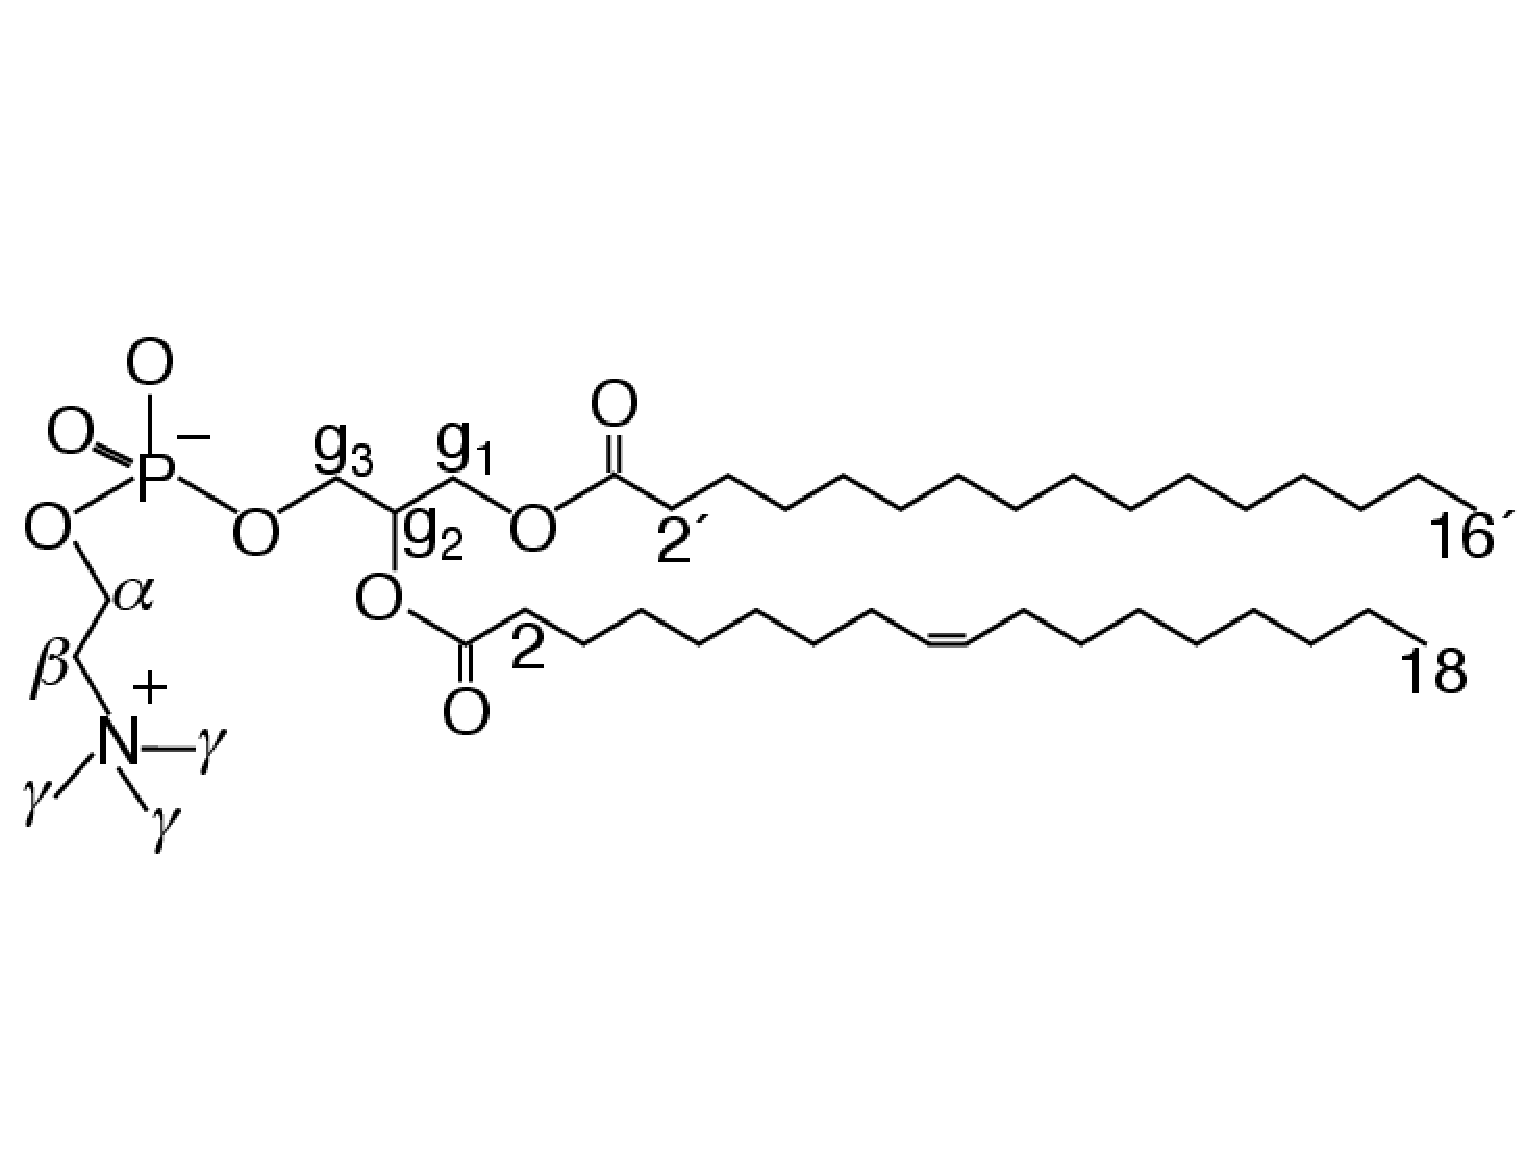
\includegraphics[width=8.6cm]{../Fig/POPCstructure.eps}

  \caption{\label{POPCstructure}
    Chemical structure of 1-palmitoyl-2-oleoylphosphatidylcholine (POPC).}
  
\end{figure}

\section{Results and Discussion}
The electrometer concept is based on the observed systematic absolute value increase for $\beta$ 
and decrease for $\alpha$ segment order parameter with inceased cation binding and {\it vice versa} for 
anions~\cite{akutsu81,altenbach84,seelig87,scherer89}. Only absolute values of the  
order parameters were measured in original experiments, while later experiments revealed that the 
order parameter is negative for $\beta$ segment and positive for $\alpha$ segment~\cite{hong95a,hong95b,gross97}. 
Thus the both order parameter values are actually decreasing (becoming more negative) with bound
cations \cite{ollila15}. The sign corrected choline order parameter changes for
POPC and DPPC bilayers as a function NaCl and CaCl$_2$ concentrations, measured with H$ 2$ 
NMR~\cite{akutsu81,altenbach84}, are shown in Fig.~\ref{ordPions}.
Only minute decreases are measured with NaCl while order of magnitude larger effect is observed
with CaCl$_2$. Interpreted in terms of the electrometer concept, the result indicate 
negligible binding of monovalent Na$^+$ ions in constrast to multivalent Ca$^{2+}$ 
ions~\cite{akutsu81,altenbach84}, in agreement with several other experimental 
studies \cite{cevc90,tocanne90,binder02,pabst07,filippov09}
\begin{figure*}[]
  \centering
  \includegraphics[width=15cm]{../Fig/OrderParameterIONSchanges.eps}
  \caption{\label{ordPions}
    The order parameter changes for $\beta$ and $\alpha$ segments as a function of NaCl (left column) 
    and CaCl$_2$ (right column) concentrations from simulations and experiments~\cite{akutsu81} 
    (POPC with CaCl$_2$ from \cite{altenbach84}). The signs of the experimental order parameters, taken from
    experiments without ions~\cite{hong95a,hong95b,gross97}, can be assumed to be unchanged 
    with concentrations represented here~\cite{altenbach84,ollila15}. It should be noted that
    none of the models used here reproduces the order parameters within experimental error
    for pure PC bilayer wihtout ions, indicating structural inaccuracies with varying severity
    for all models \cite{botan15}.
   }
\end{figure*}

Also order parameter changes with NaCl and CaCl$_2$ concentrations from various simulation models are shown in Fig.~\ref{ordPions}. 
The simulation details are in Table~\ref{IONsystems} and in Supplementary Information. 
The order parameter decrease with penetrating cations is observed in all simulation models in line with experiments.
This indicates that the choline qualitative structural response can be reproduced in simulations despite of 
inaccuracies with varying severity in the choline and glycerol backbone structures, in agreement
with our recent results with dehydration~\cite{botan15}.

%In our recent work, we showed that the experimental order parameters for choline and glycerol backbone were not
%quantitatively reproduced by any available lipid model in fully hydrated conditions, however, the response of the choline order parameters
%to dehydration were qualitatively correct in all 
%\todo{Markus: This 'all' gives the impression that it is the same as the 'any available' 
%in the beginning of the sentence. I propose we make it clear here that we only tested four FFs against dehydration.} 
%models, and the response to the cholesterol  content
%was qualitatively correct in the CHARMM36 model~\cite{botan15}. 
%\todo{Markus: Wouldn't you say that the response of the choline order parameters to cholesterol 
%content was qualitatively just as correct in MacRog as it was in CHARMM36? (Fig.~9 in Ref.~\cite{botan15})} 


To study the correlation between order parameter changes and ion partitioning into a bilayer, 
suggested by the electrometer concept~\cite{akutsu81,altenbach84,seelig87,scherer89}, the ion 
density distributions from different simulation models as a function of membrane normal with NaCl and CaCl$_2$ are shown in 
Figs.~\ref{NAdensities} and~\ref{CAdensitiesCLEAR}, respectively. The density profiles from different models in Fig.~\ref{NAdensities}
are arranged to increasing order according to the changes observed in order parameters with NaCl concentration in Fig.~\ref{ordPions}
such that the model with smallest change is on top and towards the bottom are models with larger observed order parameter changes.
The Fig.~\ref{ordPions} clearly shows that the larger Na$^+$ density peaks at the lipid bilayer interface are
observed towards the bottom of the figure correlating with the increased order parameter change. 
Thus the Na$^+$ ion binding affinity is clearly related to the $\alpha$ and $\beta$ order parameter
changes in simulations are well, thus the electrometer concept~\cite{akutsu81,altenbach84,seelig87,scherer89}
can be used to compare the Na$^+$ ion binding affinity between simulations are experiments.
This applies to all studied models despite of the varying quality of the sampled choline and glycerol backbone structures~\cite{botan15}.
The Ca$^{2+}$ penetration and related order parameter decrease is seen with all simulation models.
\begin{figure}[]
  \centering
  \includegraphics[width=8cm]{../Fig/NAdensities.eps}
  \caption{\label{NAdensities}
    Number density profiles for lipids, Na$^+$ and Cl$^-$ ions from simulations with different force fields and different NaCl concetrations. 
    The force fields are ordered according to the order parameter changes observed in Fig.~\ref{ordPions} such that the models with smallest
    observed changes are top.
    The lipid densities are scaled with 100 (united atom) or 200 (all atom model) to make them visible with the used y-axis scale.
    Figure discussed in https://github.com/NMRLipids/lipid\_ionINTERACTION/issues/4.
  }
  \todo{We need compatible data for Slipids. This is easy to calculate by modifying the current scripts, if the 
    data is available.
}
\end{figure}
\begin{figure}[]
  \centering
  \includegraphics[width=8cm]{../Fig/CAdensitiesCLEAR.eps}
  \caption{\label{CAdensitiesCLEAR}
    Number density profiles for lipids, Ca$^{2+}$ and Cl$^-$ ions from simulations with different force fields.
    The profiles only with smallest available CaCl$_2$ concentration are shown for clarity.
    Figure including all the available concetrations is shown in the Supplementary Information.
    The lipid densities are scaled with 100 (united atom) or 200 (all atom model) to make them visible with the used y-axis scale.
    Figure discussed in https://github.com/NMRLipids/lipid\_ionINTERACTION/issues/4.
  }
\end{figure}


The smallest order parameter changes in best agreement with experiments with NaCl concentration are seen for the Orange,
CHARMM36 and Lipid14 models in Fig.\ref{ordPions}. However, the ion density profiles in Fig.~\ref{NAdensities} show 
detectable differences in Na$^+$ affinity between these models, Orange having lowest affinity and CHARMM36 highest. 
None of the models reproduces all the order parameters in Fig.~\ref{ordPions} within experimental error and 
these very small order parameter changes (less than 0.02) may be delicate to, e.g. initial structures.
Thus we cannot conclude if one of these three models is more realistic than another, especially with physiological
NaCl concentrations ($\sim$ 150mM) which is most relevant for most applications. On the other hand, all
the other studied models clearly overestimate the choline order parameter changes respect to experiments, as seen from Fig.~\ref{ordPions}.
This is related to the unrealistically strong Na$^+$ binding to the bilayer, evidenced by the density peaks 
in Fig.~\ref{NAdensities} which are seen also with physiological concentrations. 

It is agreed in the literature that the Ca$^{2+}$ ions do penetrate in the phosphatidylcholine bilayer and
significantly affect membrane properties already at mM concentrations of CaCl$_2$, however, the strength of 
the binding is not agreed on~\cite{tatulian87,altenbach84,bockmann04}.
\todo{Markus: Mention shortly what strengths have been suggested?}
The binding and related order parameter decrease are seen in all tested models in Figs. \ref{ordPions} and \ref{CAdensitiesCLEAR}.
However, the order parameter changes are overestimated in all models in respect to the experiments,
thus none of these models cannot be used to interpret the Ca$^{2+}$ induced structural changes to the
lipids or number of bound lipids. In contrast to the Na$ +$, there is no clear correlation between Ca$^{2+}$
binding affinity and order parameter changes, thus the overestimation of order parameter change can be 
due to, e.g. too strong strong binding, incorrect headgroup response to penetrating divalent cation or 
penetration depth. The penetration depth of Ca$^{2+}$ ions is similar (density maxima close to $\pm$2 nm) 
in all models except Berger with deeper penetration depth (density maxima close to $\pm$1.8 nm).  
The location closer to water phase is probably more realistic since $^1$H NMR and neutron scattering data 
indicates that Ca$^{2+}$ interact mainly with choline group~\cite{hauser76,hauser78,herbette84,cevc90}.
Further, the $^1$H NMR experiments suggest that the N-$\beta$-$\alpha$-O dihedral is only in 
gaughe--conformation in the absense of ions, but in the presense of multivalent ions also anti--conformations
would be present \cite{hauser78, hauser81}. However, since the models reproduce the conformations 
without ions with varying quality and the experimental order parameter response to CaCl$_2$ concentration
current MD models cannot used to interpret this.
%I have now calculated the dihedral distributions for this dihedral with different CaCl$_2$ concentrations in different models, see Fig.~\ref{ObaNdihs}.
%The change suggested by the $^1$H NMR experiments is not seen in the CHARMM36 model. In Orange model this dihedral is mostly in anti
%conformation also without CaCl$_2$, oppositely as suggested by $^1$H NMR experiments. With CaCl$_2$ anti conformations become slightly more
%pronounced, however, the conformation seems to be unrealistic from the beginning so the studies of structural response to the CaCl$_2$
%might not be reasonable with this model. I think we need more simulations with CHARMM36 to see how good the order parameter response
%to the CaCl$_2$ actually is. Then we can discuss more about its structural response.} \\
\todo{The P-N vector tilting analysis should be considered}



%\begin{figure}[]
%  \centering
%  \includegraphics[width=8cm]{../Fig/OrderParameterIONSnaclSIGN.eps}
%  \caption{\label{ordPnacl}
%    Order parameters as a function of NaCl concentration from simulations 
%     with the Berger, CHARMM36, MacRog and Orange force fields compared to the experiments
%     by Akutsu et al.~\cite{akutsu81} and Altenbach et al.~\cite{altenbach84}. The signs are assumed to be the same as measured by Hong et al.~\cite{hong95a}, Hong et al.~\cite{hong95b} and Gross et al.~\cite{gross97}. 
%     The experimental data for the effect of ions to the glycerol backbone is not found, thus only the values without ions are shown. 
%     The straight line between the results with and without ions is plotted to guide the eye. 
%   }
%\todo{Samuli: I think that this figure could be removed. This is very unclear and I think would be difficult to make
%more clea. I am thinking that we could show the order parameters for pure bilayer compared to experiments 
%(as in the first paper) to remind the quality different models without ions. And the show only the changes
%as a function of ions. Issue discussed here: https://github.com/NMRLipids/lipid\_ionINTERACTION/issues/3
%
%Markus: Also, is there any point in showing the glycerol values as a function of [NaCl], if we do not have experimental data to compare against?}
%\end{figure}

%\begin{figure}[]
%  \centering
%  \includegraphics[width=8cm]{../Fig/OrderParameterIONSCaCl.eps}
%  \caption{\label{ordPcacl}
%    Order parameters as a function of CaCl concentration from simulations 
%     with the Berger 
%CHARMM36, MacRog 
%and Orange force fields compared to the experiments by Akutsu et al.~\cite{akutsu81} and Altenbach et al.~\cite{altenbach84}. 
%The signs are assumed to be the same as measured by Hong et al.~\cite{hong95a}, Hong et al.~\cite{hong95b} and Gross et al.~\cite{gross97}. 
%     The effect of ions to the g1 and g2 were not measured, thus only the values without ions are shown. The straight line between the results with and without ions is 
%     plotted to guide the eye. }
%\todo{I think that this figure could be removed as the previous. Issue discussed here: https://github.com/NMRLipids/lipid\_ionINTERACTION/issues/3}
%\end{figure}

\begin{table*}[htb]
\centering
\caption{Simulated lipid bilayers with ions. The ion concentrations are the concentration of 
  ions in buffer to solute the lipid bilayers and calculated as [ion]=(N$_{\rm ion} \times$[water])/N$_{\rm w}$, 
  where [water]=55.5M. These correspond the concentrations reported in the experiments by Akutsu et al.~\cite{akutsu81}.}\label{IONsystems}
\begin{tabular}{c c c c c c c c c c c c}
  %\hline
  Force field (lipid/ion)& lipid & [Ion] mM & \footnote{The number of lipid molecules}N$_{\rm l}$   &  \footnote{The number of water molecules}N$_{\rm w}$   & \footnote{The number of Na$^+$ molecules}N$_{\rm Na}$  & \footnote{The number of Ca$^{2+}$ molecules}N$_{\rm Ca}$   &  \footnote{The number of Cl molecules}N$_{\rm Cl}$ & \footnote{Simulation temperature}T (K)  & \footnote{The total simulation time}t$_{{\rm sim}}$(ns) & \footnote{Time frames used in the analysis}t$_{{\rm anal}}$ (ns) & Files\\
  \hline
  Berger-POPC-07\cite{ollila07a}   &   POPC & 0          & 128 & 7290 & 0  & 0  & 0 & 298  & 270 & 240 & \cite{bergerFILESpopc}  \\
  Berger-POPC-07\cite{ollila07a}/Gromos~\cite{??}\todoi{Appropriate reference for the ion model?}   &   POPC & 340 (NaCl) & 128 & 7202 & 44  & 0  & 44 &298  & 110 & 50 & \cite{bergerPOPC340mMNaClfiles} \\
  %\hdashline
  Berger-POPC-07\cite{ollila07a}/Gromos~\cite{??}\todoi{Appropriate reference for the ion model?}   &   POPC & 340 (CaCl$_2$) & 128 & 7157 & 0 & 44  & 88 &298 & 108 & 58 &\cite{bergerPOPC340mMCaClfiles}  \\
  \hline
  Berger-DPPC-98\cite{marrink98}   &   DPPC & 0 & 72 & 2880 & 0  & 0  & 0 &323  & 60 & 50 &\cite{bergerDPPCfiles} \\
  Berger-DPPC-98\cite{marrink98}/Gromos~\cite{??}   &   DPPC & 0 & 72 & 2880 & 8  & 0  & 8 &323  & 120 & 60 &\cite{bergerDPPC150mMfiles} \\
  Berger-DPPC-98\cite{marrink98}/Gromos~\cite{??}   &   DPPC & 1000 (NaCl) & 72 & 2778 & 51  & 0  & 51 &323  & 120 & 60 &\cite{bergerDPPC1000mMfiles} \\
  \hline
  BergerOPLS-DPPC-06\cite{tieleman06} &   DPPC & 0 & 72 & 2880 & 0  & 0  & 0 &323  & 120 & 60 &\cite{bergerOPLSDPPCfiles} \\
  BergerOPLS-DPPC-06\cite{tieleman06}/\r{A}qvist~\cite{aqvist90} &   DPPC & 150 & 72 & 2880 & 8  & 0  & 8 &323  & 120 & 60 &\cite{bergerOPLSDPPCfiles150mMnacl} \\
  BergerOPLS-DPPC-06\cite{tieleman06}/\r{A}qvist~\cite{aqvist90} &   DPPC & 1000 & 72 & 2778 & 51  & 0  & 51 &323  & 120 & 60 &\cite{bergerOPLSDPPCfiles1000mMnacl} \\
  \hline
  CHARMM36\cite{klauda10}   & POPC & 0           & 72 & 2242 & 0  & 0 & 0 & 303  & 30 & 20 & \cite{charmm36filesSHORT} \\
  CHARMM36\cite{klauda10}/ionFF~\cite{venable13} & POPC & 350 (NaCl)  & 72 & 2085 & 13  & 0 & 13 & 303  & 80 & 60 & \cite{charmmPOPC350mMNaClfiles} \\
  CHARMM36\cite{klauda10}/ionFF~\cite{venable13} & POPC & 690 (NaCl)  & 72 & 2085 & 26  & 0 & 26 & 303  & 73 & 60 & \cite{charmmPOPC690mMNaClfiles}   \\
  CHARMM36\cite{klauda10}/ionFF~\cite{venable13}  & POPC & 950 (NaCl)  & 72 & 2168 & 37  & 0 & 37 & 303  & 80 & 60 &\cite{charmmPOPC950mMNaClfiles}  \\
  %CHARMM36\cite{klauda10}, ionFF~\cite{??}\todoi{Appropriate reference for the ion model?}  & POPC & 1380 (NaCl)  & 72 & 2085 & 52  & 0 & 52 & 303  & 80 & 60 &?\todoi{Samuli put to Zenodo} \\
  %CHARMM36\cite{klauda10}, ionFF~\cite{??}\todoi{Appropriate reference for the ion model?}   & POPC & 2080  (NaCl)  & 72 & 2085 & 78  & 0 & 78 & 303  & 73 & 60 &?\todoi{Samuli put to Zenodo} \\
  CHARMM36\cite{klauda10}/ionFF~\cite{??} & POPC &  350 (CaCl$_2$)  & 128 & 6400 & 0& 35 & 70 & 303  & 200  & 100 & \cite{charmmPOPC350mMCaClfiles}  \\
  CHARMM36\cite{klauda10}/ionFF~\cite{??} & POPC &  670 (CaCl$_2$)  & 128 & 6400 & 0& 67 & 134 & 303  & 200  & 120 & \cite{charmmPOPC670mMCaClfiles}  \\  
  CHARMM36\cite{klauda10}/ionFF~\cite{??} & POPC &  1000 (CaCl$_2$) & 128 & 6400 & 0& 100 & 200 & 303 & 200  & 100 & \cite{charmmPOPC1000mMCaClfiles}  \\
  \hline
  MacRog\cite{maciejewski14}  & POPC & 0 & 288 & 14400 & 0 & 0 & 0 & 310 & 90&40  &~\cite{macrogdehydFILES}  \\
  MacRog\cite{maciejewski14}/ionFF~\cite{??}\todoi{Appropriate reference for the ion model?}  & POPC & 100 (NaCl) & 288 & 14554 & 27 & 0 & 27 & 310 & 90&50  & \cite{macrogIONfiles} \\
  MacRog\cite{maciejewski14}/ionFF~\cite{??}\todoi{Appropriate reference for the ion model?}        & POPC &  210 (NaCl) & 288 & 14500 & 54 & 0 & 54 & 310 & 90&50  &\cite{macrogIONfiles}  \\
  MacRog\cite{maciejewski14}/ionFF~\cite{??}\todoi{Appropriate reference for the ion model?}        & POPC &   310 (NaCl) & 288 & 14446 & 81 & 0 & 81 & 310 & 90&50  & \cite{macrogIONfiles} \\
  MacRog\cite{maciejewski14}/ionFF~\cite{??}\todoi{Appropriate reference for the ion model?}        & POPC &   420 (NaCl) & 288 & 14392 & 108 & 0 & 108 & 310 & 90& 50  & \cite{macrogIONfiles}  \\
  \hline
  Orange, ionFF~\cite{??}  &   POPC & 0 & 72 & 2880 & 0 & 0  & 0 & 298 & 60 & 50 & \cite{orangePOPCfiles}  \\
  Orange, ionFF~\cite{??}\ &   POPC & 140 (NaCl) & 72 & 2866 & 7 & 0  & 7 & 298 & 120 & 100 &\cite{orangePOPC140mMNaClfiles}  \\
  Orange, ionFF~\cite{??}\todoi{Appropriate reference for the ion model?}   &   POPC & 510 (NaCl) & 72 & 2802 & 26 & 0  & 26 & 298 & 120 & 100 &\cite{orangePOPC510mMNaClfiles}   \\
  Orange, ionFF~\cite{??}  &   POPC & 1000 (NaCl) & 72 & 2780 & 50 & 0  & 50 & 298 & 120 & 80 & \cite{orangePOPC1000mMNaClfiles} \\
  %\hdashline
  Orange, ionFF~\cite{??}\todoi{Appropriate reference for the ion model?}   &   POPC & 510 (CaCl$_2$)  & 72 & 2802 & 0 & 26  & 52 & 298 & 120 & 60 & \cite{orangePOPC510mMCaClfiles}  \\
  \hline
  Slipid\cite{jambeck12}   &   DPPC & 0 & 128 &3840 & 0 & 0  & 0 & 323 & 150 & 100 &~\cite{slipidsFILES}  \\
  Slipid\cite{jambeck12}, ionFF~\cite{??}\todoi{Andrea Catte, please let us know if you share some files through Zenodo}    &   DPPC & 150 (NaCl) & 600 & 18000 & 49 & 0  & 49 & 323 & 100 & 40 &?  \\
  \hline
  Lipid14/AMBER99SB-ILDN\cite{??}   &   POPC & 0          & 128 & 5120 & 0 & 0  & 0 & 298 & 205 & 200 &~\cite{lipid14POPC0mMNaClfiles}  \\
  Lipid14/AMBER99SB-ILDN\cite{??}   &   POPC & 150 (NaCl) & 128 & 5120 & 12 & 0 & 12 & 298 & 205 & 200 &~\cite{lipid14POPC150mMNaClfiles}  \\
  Lipid14/AMBER99SB-ILDN\cite{??}   &   POPC & 1000 (NaCl) & 128 & 5120 & 77 & 0 & 77 & 298 & 205 & 200 &~\cite{lipid14POPC1000mMNaClfiles}  \\
  Lipid14/AMBER99SB-ILDN\cite{??}   &   POPC & 350 (CaCl$_2$) & 128 & 6400 & 0 & 35 & 70 & 298 & 200 & 100 &~\cite{lipid14POPC350mMCaClfiles}  \\
  Lipid14/AMBER99SB-ILDN\cite{??}   &   POPC & 1000 (CaCl$_2$) & 128 & 6400 & 0 & 100 & 200 & 298 & 200 & 100 &~\cite{lipid14POPC1000mMCaClfiles}  \\
  \hline
  Ulmschneiders/OPLS\cite{??}       &   POPC & 0          & 128 & 5120 & 0 & 0  & 0 & 298.15 & 205 & 200 &~\cite{ulmschneiderPOPC0mMNaClfiles}  \\
  Ulmschneiders/OPLS\cite{??}       &   POPC & 150 (NaCl) & 128 & 5120 & 12 & 0  & 12 & 298.15 & 205 & 200 &~\cite{ulmschneiderPOPC150mMNaClfiles}  \\
  Ulmschneiders/OPLS\cite{??}       &   POPC & 1000 (NaCl) & 128 & 5120 & 77 & 0  & 77 & 298.15 & 205 & 200 &~\cite{ulmschneiderPOPC1000mMNaClfiles}  \\
\end{tabular}
\end{table*} 

%The most important observation is that the experimental order parameters for the headgroup and glycerol bakcbone g$_3$ segment 
%\todo{Markus: There seems to be NO experimental g$_3$ data in Fig.~\ref{ordPnacl}...}
%are practically unhanged even though 1M NaCl concentration was added to the system. Thus, the presence of mM concentrations
%of NaCl does not affect the structure of these parts of lipids. Thus, the most straightforward explanation for the experimental results shown
%in Fig.~\ref{ordPnacl} is that the Na$^+$ and Cl$^-$ ions do not essentially penetrate into a phospholipid bilayer below 1M concentrations.

%The response of order parameters to the NaCl concentration in simulations depends on the used model in Fig.~\ref{ordPnacl}:
%The addition of NaCl leads to a significant changes for choline and $g_2$ and g$_3$ segments in glycerol bakcbone
%in Berger and MacRog models, while only moderate changes are seen in CHARMM36 and Orange force fields.
%The experimental data for glycerol backbone as a function of NaCl concentration is available only for the
%g$_3$ segment. \todo{Markus: For some reason, these g$_3$ data are not shown in Fig.~\ref{ordPnacl}} 
%The changes in g$_1$ and g$_2$ are unlikely since all the other order parameters are unaffected
%and 


The most straightforward explanation for our results is that Na$^+$ ions do not practically penetrate into a PC lipid bilayer
at mM concentrations, thus the presense of NaCl does not affect the bilayer properties as observed in various 
experiments~\cite{akutsu81,altenbach84,clarke99,binder02,pabst07,filippov09}.
Consequently, the Na$^+$ penetration and concominant changes in order parameters, area per molecule and lateral diffusion 
seen in almost all simulation models would be artefact due to overestimated attraction between ions and lipid bilayer.
Even though this would also explain the absense of positive zeta potential in electrophoresis 
experiments~\cite{eisenberg79,tatulian87,manyes05,manyes06,klasczyk10},  
the presented data do not rule out the suggested possibility of equal binding of Na$^+$ and Cl$^-$ ions~\cite{knecht13},
however, this equal binding should happen in such a way that the bilayer properties are unaffected.
The negligible binding of Na$^+$ at mM concentrations suggested here differs from the conclusions made from 
measurements of fluorescent probe dynamics~\cite{bockmann03,vacha09a,harb13}, membrane hardness with 
AFM~\cite{manyes05,manyes06,fukuma07,ferber11,morata12} and calorimetry~\cite{bockmann03,klasczyk10}.
However, the fluorescent measurement results may arise from direct interactions between probe and ions, as already 
suggested by Filippov et al.~\cite{filippov09}. 
Further, the calorimetric results have been also interpreted to support negligible binding~\cite{cevc90}, 
and AFM result is relatively indirect, thus there may be alternative explanations as well.


%In conclusion, our results show that the Na$^+$ association to PC bilayer is significantly too strong in the Berger and MacRog models,
%while Orange and CHARMM36 force fields predict more realistic binding affinity. Since some modest changes are also seen in 
%Orange and CHARMM36 results, more careful simulation studies would be needed to judge if the Na$^+$ association is slightly 
%too strong also in these  models. The stonger Na$^+$ ion association in GROMOS based force fields compared to CHARMM based force 
%has been already reported in the literature~\cite{berkowitz06,cordomi09,valley11,berkowitz12,sachs04,valley11},
%however the novelty of this work in this respect is that we make a direct comparison
%to the experiments which can be used as measure for the model quality. 

The origin for suggested inaccuracies in lipid-ion interactions in simulation models is unknown. 
In principle, the incorrect choline structure~\cite{botan15}, lack of polarizability~\cite{leontyev11} or
the used water model could cause such results. The effect of changes in lipid and ion models on the ion
partitioning is discussed in the supplementary material.
\todo{In the Orange simulation only lipid model is changed, respect to Berger, and Jukka tested the effect
of 0.7 charge scaling for Na ion (suggested by Leontyev et al.~\cite{leontyev11} to compensate to the lack 
of electronic polarizability in the model). I think we should discuss these things in supplementary material.
Even though we cannot be fully conclusive, there is some essential information also in these results.} 

The failure
 of Gromos ions to properly account ion--ion and ion--water binding propensities of Na$^+$ and Cl$^-$ ions has been
 reported previously~\cite{Reif13}. The \r{A}qvist ions have been parameterized in aqueous solutions with good agreement
 to experimental energies~\cite{Aaqvist90}. Yet, the binding affinity of ions to lipid bilayers has not been
 calibrated---instead it is assumed to work based purely on forces obtained using combination rules. Compared to Gromos
 ions, \r{A}qvist parameters are better, yet Na$^+$ overbinding still occurs.


%From the technical point of view it is interesting to note that the same ion model is used in the Berger and Orange simulation, only difference 
%being in the lipid model, indicating that the partitioning can be strongly reduced just by modifying the lipid
%model parameters. 

%In situations where a positive charge penetrates into a bilayer (e.g. cationic surfactant~\cite{scherer89} or multivalent ion~\cite{akutsu81}) 
%a decrease in choline order parameters is observed in experiments, as also seen in CaCl$_2$ results in Fig.~\ref{ordPions}.
%Also in all simulations analyzed in this work where cation is penetrating into a bilayer, the choline order parameters
%decrease as seen in Fig.~\ref{ordPions}. However, in the case of CaCl$_2$ the decrease in too pronounced in 
%simulations which may arise from too strong partitioning of Ca$^{2+}$ or overestimated influence of charge on lipid conformation.

\section{Conclusions}
We have compared phosholipid bilayer interactions with NaCl and CaCl$_2$ between different molecular dynamics simulation
models and $^2$H NMR experiments. The comparison led to the following conclusions

- The electrometer concept suggesting connection between $\alpha$ and $\beta$ order parameter decrease and
cation partitioning~\cite{akutsu81,altenbach84,seelig87,scherer89} works also in simulations, despite of inaccuracies in actual atomistic resolution structures. 

- The most straighforward explanation for the various experimental observations is that there is no Na$^+$ ion binding
into the phospholipid bilayer at mM concentrations, in constrast to Ca$^{2+}$ which specifically binds.

- The Na$^+$ partitioning is overestimated in almost all molecular dynamics simulation models, however, from the publicly available models the CHARMM36 has the most realistic description.

%Our discussion gives further support to the idea that choline orientation and ion partitioning can
%be experimentally measured by using the choline group order parameters as suggested in the series of
%publications by Seelig and co workers.
%However, we have updated the details of the relation by including the information about 
%the sings.

- \todo{Final conclusions about the structural response to be written once we have all the results} 


%In conclusion, the penetrating induced decrease in order parameters can be seen in all models
%independently of the detailed molecular structure in the model, corresponding to the dehydration case
%where increase was seen in all models. The most likely explanation is that, despite of the structural model, the choline group
%orients more parallel to the membrane normal with penetrating cations. In contrast to the dehydration results,
%we are not aware of experimental data for the glycerol order parameters as a function of penetrating ions. 
%Furher, our results show that the Na$^+$ partitioning into a PC bilayer with Berger model is a
%simulation artefact, thus the research lines based these results should be taken with caution.


%This work has been done, and will be progressed, as an open collaboration through nmrlipids.blogspot.fi.






%Similar significant structural changes in the headgroup region are seen upon the addition
%of sodium and calcium ions in the Berger model. This contradicts with the experiments where
%sodium does not change the headgroup structure and the changes observed for calcium are different from those seen in simulations.
%These results indicate that the changes in the headgroup structure due to a permeating charge are not correct
%in the Berger model and, in particular, that sodium ions penetrating the headgroup region is erroneous.

This work has been, and will be, progressed and discussed through the blog: nmrlipids.blogspot.fi. 
Everyone is invited to join the discussion and make contributions through the blog. 
The manuscript will be eventually submitted to an appropriate scientific journal. 
Everyone who has contributed to the work through the blog will be offered 
coauthorship. For more details see: nmrlipids.blogspot.fi.   

{\bf Acknowledgements: }
OHSO acknowledges Tiago Ferreira for very useful discussions, the Emil Aaltonen foundation for financial support, Aalto Science-IT project and CSC-IT Center for Science for computational resources. 
%
MSM acknowledges financial support from the Volkswagen Foundation (86110).

\newpage

\appendix
\begin{center}
{\bf SUPPLEMENTARY INFORMATION}
\end{center}

\section{Effect of ion model and polarization}

 We also tested if different ion models and implicit accounting of polarization would affect ion binding.
% Changing the model description from Berger-DPPC-98~\cite{Marrink98} and Gromos ion
% parameters~\cite{??}\todoi{Appropriate reference for the ion model?} to OPLS-AA compatible
% Berger-DPPC-06~\cite{tieleman06} and \r{A}qvist ions~\cite{Aaqvist90} results in slightly decreased ion binding affinity
% as seen from the density plots in Figure \ref{ionnotscaled}~\cite{DPPCBergerNaCl,bergerOPLSDPPCfiles150mMnacl}. 
To compensate the missing electronic polarizability, Leontyev et al.~\cite{leontyev11} have suggested
that ion charges should be scaled by a factor of 0.7. To test if this scaling alone could correct the ion
binding affinity we ran simulations with scaled ion charges with Berger-DPPC-98 and BergerOPLS-DPPC-06 models 
(the systems identical as in Table~\ref{IONsystems} except that the ion charges are scaled with 0.7, the files available 
at ~\cite{DPPCBergerNaCl150mMscaled,DPPCBergerNaCl1000mMscaled,DPPCBergerOPLS06NaCl150mMscaled,DPPCBergerOPLS06NaCl1000mMscaled}). 
The order parameter changes and ion affinity are smaller with scaled charges but yet overestimated respect to
the experiments as seen from Figs. \ref{OPchangesSCALED} and~\ref{NAdensitySCALED}. Thus the overestimated
binding affinity cannot be fixed by only scaling charges.


%The intuitive explanation is that by scaling the partial charges the charge discrepancy between the ion and water partial charges is decreased. This means
%that there is a lesser driving force for ions to bind to the highly-charged phosphate group. Furthermore, with
%Berger-DPPC-06 and scaled \r{A}qvist ions (Q=0.7) we obtain that there is only very weak binding of sodium to DPPC as
%observed experimentally (right side of Figure \ref{ionscaled}). In scaled models the order parameter changes 
%are also small. However, the ion concentration is also small. To be fully conclusive, if the affinity can be fixed by scaling,
%we need to run simulations also with large concentrations.


%The results indicate that the polarization effect actually improves ion binding affinities irrespectively of the model.
%However, the drawback of the scaled charges is that the total charge of the simulation box is non-zero whenever
%counterions and charged molecules are present. This may cause simulation artefacts. Even though in methods such as
%PME the residual charge does not affect the forces (and thus dynamics), it still has an effect to the energies.
%This is because the potential from the residual charge is 'smeared in the box' and so depends on the possibly
%fluctuating (at least in NPT conditions) volume of the simulation box. 

\begin{figure}[]
  \centering
  \includegraphics[width=8cm]{../Fig/OrderParameterIONSchangesSCALED.eps} %https://zenodo.org/record/16319/files/density.png
  \caption{\label{OPchangesSCALED}
    Order parameter changes in scaled and non-scaled models. The Berger-OPLS compatible model results are missing since there are
    no results without ions for this.
}
\end{figure}

\begin{figure}[]
  \centering
  \includegraphics[width=8cm]{../Fig/NAdensitiesSCALED.eps} %https://zenodo.org/record/16319/files/density.png
  \caption{\label{NAdensitySCALED}
    Number density profiles for lipids, Na$^+$ and Cl$^-$ ions from simulations with different force fields and different NaCl concetrations. 
    The ion charges are scaled with 0.7 to compensate the missing electronic polarizability~\cite{leontyev11}.
    The lipid densities are scaled with 100 (united atom) or 200 (all atom model) to make them visible with the used y-axis scale.
}
\end{figure}


%\begin{figure*}[]
%  \centering
%  \includegraphics[width=0.49\textwidth]{../Fig/ionnotscaledberger98.eps} %https://zenodo.org/record/16319/files/density.png
%  \includegraphics[width=0.49\textwidth]{../Fig/ionnotscaledberger06.eps} %https://zenodo.org/record/16484/files/density.png
%  \caption{\label{ionnotscaled}
%    Density plots of DPPC bilayer and ions. DPPC density has been scaled down by a factor of 100 for clarity. Left: Berger-DPPC-98 model with Gromos ions. Right: Berger-DPPC-06 model with \r{A}qvist ions.
%}
%\end{figure*}
%Raw data in .xvg format for this figure can be found at
%https://zenodo.org/record/16319/files/ and https://zenodo.org/record/16384/files/

%\begin{figure*}[]
%  \centering
%  \includegraphics[width=0.49\textwidth]{../Fig/ionscaledberger98.eps} %https://zenodo.org/record/16320/files/density.png
%  \includegraphics[width=0.49\textwidth]{../Fig/ionscaledberger06.eps} %https://zenodo.org/record/16485/files/density.png
%  \caption{\label{ionscaled}
%   Density plots of DPPC bilayer and polarization corrected ions, where ion charges are scaled by 0.7. DPPC density has been scaled down by a factor of 100 for clarity. Left: Berger-DPPC-98 model with scaled Gromos ions. Right: Berger-DPPC-06 model with scaled \r{A}qvist ions.
%   }
%\end{figure*}
%Raw data in .xvg format for this figure can be found at
%https://zenodo.org/record/16320/files/ and https://zenodo.org/record/16385/files/

\section{Structural changes induced by CaCl$_2$}
\begin{figure}[]
  \centering
  \includegraphics[width=8cm]{../Fig/CAdensities.eps}
  \caption{\label{CAdensities}
    Number density profiles for lipids, Ca$^{2+}$ and Cl$^-$ ions from simulations with different force fields 
    and different CaCl$_2$ concentrations. 
    The lipid densities are scaled with 100 (united atom) or 200 (all atom model) to make them visible with the used y-axis scale.
    Figure discussed in https://github.com/NMRLipids/lipid\_ionINTERACTION/issues/4.
  }
\end{figure}

\begin{figure*}[]
  \centering
  \includegraphics[width=0.49\textwidth]{../Fig/O-b-a-NdihWITHcaCHARMM36.eps} %https://zenodo.org/record/16320/files/density.png
  \includegraphics[width=0.49\textwidth]{../Fig/O-b-a-NdihWITHcaORANGE.eps} %https://zenodo.org/record/16485/files/density.png
  \caption{\label{ObaNdihs}
      Dihedral angle distributions for O-$\beta$-$\alpha$-N dihedral with different CaCl$_2$ concentrations.}
\end{figure*}

%The order parameters calculated from previously published quadrupolar splitting data were calculated using 
%the equation $|S_{{\rm CD}}|=0.00784 \times \Delta \nu_Q$, where $\Delta \nu_Q$ is the quadrupolar splitting measured
%by $^2$H NMR (for more details see~\cite{seelig77c} and supplementary information).
%The order parameters measured with $^{13}$C NMR were calculated from dipolar splitting by using equation
%$|S_{{\rm CH}}|=\frac{4\pi\langle r_\mathrm{CH}^3 \rangle}{\hbar \mu_0 \gamma_h \gamma_c} d_\mathrm{CH}$, where
%$d_\mathrm{CH}$ is the measured dipolar splitting and
%values between 20.2-22.7 kHz were used for $\frac{4\pi\langle r_\mathrm{CH}^3 \rangle}{\hbar \mu_0 \gamma_h \gamma_c}$,
%depending on the original authors~\cite{hong95a,gross97,dvinskikh05,ferreira13} (for more discussion see supplementary material).


\section{methods}

\subsection{Simulated systems}
All simulations are ran with a standard setup for planar lipid bilayer in zero tension
with periodic boundary conditions with Gromacs software package (version numbers 4.5-X-5.0.X).
%The number of molecules, temperatures and the length of simulations for all the fully 
%hydrated lipid bilayer simulations are listed in Table~\ref{systems}. Full simulation
%details for all simulations are given the next section.

%For intitial configuration of the simulations with NaCl and CaCl$_2$, the required number of randomly placed water molecules were replaced by 
%ions in fully hydrated simulations. 
%The molar concentration was calculated as ??. 
%The number of different molecules, temperatures and 
%the length of simulations for all the ion containing simulations are show in Table~\ref{IONsystems}.


%the POPC bilayer was solvated with 7202 water molecules, 44 Na$^+$ and Cl$^-$ ions,
%corresponding roughly to [NaCl] $\approx$ 200~mM. For simulations with CaCl$_2$, the POPC bilayer was solvated with 
%7157 water molecules, 44 Ca$^{2+}$ and 88 Cl$^-$ ions, corresponding roughly to [CaCl$_2$] $\approx$ 200~mM. 
%The order parameters were calculated from the last 50~ns of a trajectory
%totalling 110~ns. 


\subsection{Simulation details}
\subsubsection{Berger}
The simulation without ions is the same as in~\cite{botan15}. The starting structures for simulations with ions is
made by replacing water molecules with appropriate amount of ions under study.
\todo{Samuli, finalize and check the methods.}

The Berger force field was used for the POPC~\cite{berger97}, with the dihedral potential next to the double bond 
taken from~\cite{bachar04}. The simulations are identical to previous publications~\cite{ollila07a,ferreira13,ferreira15}.
Timestep of 2~fs was used with leap-frog integrator. Covalent bond lengths were constrained with LINCS algorithm~\cite{hess97,hess07}. 
Coordinates were written every 10~ps. PME with real space cut-off 1.0~nm was used 
for electrostatics. Plain cut-off was used for the Lennard-Jones interactions with a 1.0~nm cut-off.
The neighbour list was updated every 5th step with cut-off 1.0~nm. Temperature was coupled separately
for lipids and water to 298~K with the velocity-rescale method~\cite{bussi07} with coupling constant 0.1~ps$^{-1}$.
Pressure was semi-isotropically coupled to the athmospheric pressure with the Berendsen method~\cite{berendsen84}.

\subsubsection{BergerOPLS}
\todo{Simulation details from Jukka M{\"a}{\"a}tt{\"a}}

\subsubsection{CHARMM36}
{\it POPC with NaCl}
The simulation without ions is taken directly from~\cite{botan15,charmm36filesSHORT}. 
The starting structures for simulations with NaCl were made by replacing randomly located 
water molecules of the structure of pure POPC simulation with appropriate amount of ions.
The force field for lipid were the same as in~\cite{botan15,charmm36filesSHORT}.
The ion parameters with NBFIX by Venable et al.~\cite{venable13} were used.
Simulations were ran with Gromacs 4.5.5 software~\cite{pronk13}.
\todo{Still to be checked}
Timestep of 1~fs was used with leap-frog integrator. Covalent bonds with hydrogens were constrained with LINCS algorithm~\cite{hess97,hess07}. 
Coordinates were written every 5~ps. PME with real space cut-off 1.4~nm was used 
for electrostatics. Lennard-Jones interactions were switched to zero between 0.8~nm and 1.2~nm.
The neighbour list was updated every 5th step with cut-off 1.4~nm. Temperature was coupled separately
for lipids and water to 303~K with the velocity-rescale method~\cite{bussi07} with coupling constant 0.2~ps.
Pressure was semi-isotropically coupled to the athmospheric pressure with the Berendsen method~\cite{berendsen84}.

%CaCl_2 simulations by MYKHAILO:
{\it POPC with CaCl$_2$}
The starting structures with varying amounts of CaCl$_2$ ions were constructed using the CHARMM-GUI Membrane Builder (http://www.charmm-gui.org/) online tool~\cite{lee15}. 
All runs were performed with Gromacs 5.0.3 software package~\cite{abraham15} and CHARMM36 additive force field parameters for lipids~\cite{klauda10} and ions~\cite{??} were obtained from CHARMM-GUI input files. 
Standard CHARMM-GUI mdp options were used. Particularly, h-bond lengths were constrained with LINCS~\cite{hess97,hess07}. The temperatures of the 
lipids and the solvent were separately coupled to the Nose-Hoover~\cite{nose84,hoover85} thermostat with a target temperature of 303 K and a relaxation time constant of 1.0 ps. Semi-isotropical 
pressure coupling to 1 bar was obtained with the Parrinello-Rahman barostat~\cite{parrinello81} with a time constant of 5 ps. Equations of motion were integrated with the Verlet algorithm~\cite{pall13} 
using a timestep of 2 fs. Long-range electrostatic interactions were calculated using the PME~\cite{darden93,essman95} method with a fourth order smoothing spline. A real space cut-off of 1.2 nm 
was employed with grid spacing of 0.12 nm in the reciprocal space. Lennard-Jones interactions were smoothly swithced to zero between 1.0 nm and 1.2 nm. Verlet cutoff-scheme~\cite{pall13}  
were used with the long-range neighbor list updated every 20 steps. Coordinates were written every 10 ps.
After energy minimization and an equilibration run of 0.5 ns, 200ns simulations were ran and the last 100ns of each simulation was employed for the analysis.

\subsubsection{MacRog}
The simulation parameters are identical to those employed in our earlier study~\cite{botan15} for the full 
hydration and dehydration simulations. The initial structures with varying amounts of NaCl were constructed from an 
extensively hydrated bilayer by replacing water molecules with ions using the Gromacs tool genion~\cite{gromacsMANUAL}. Even at the highest 
considered salt concentration, the amount of water molecules per lipid after this replacement process was still greater than 50.

\subsubsection{Orange}
\todo{Jukka Maatta and Luca Monticelli, please deliver as much details as you can.}

\subsubsection{Slipids}
The simulation without ions is the same as in~\cite{botan15}.

\todo{Add references to Slipids with ions.}
For the simulations with ions, the starting DPPC lipid bilayer, which was built with the online CHARMM-GUI
(http://www.charmm-gui.org/), contained 600 lipids, 30 water molecules/lipid, Na$^+$ and Cl$^-$ ions (150 mM NaCl). 
The TIP3P water model was used to solvate the system. All-atom MD simulations of DPPC lipid bilayers were performed 
at ten different temperatures (283, 298, 303, 308, 312, 313, 314, 318, 323, and 333 K) using the GROMACS software 
package version 4.5.5~\cite{pronk13} and the Stockholm lipids (Slipids) force field parameters for phospholipids. After energy 
minimization and a short equilibration run of 50 ps (time step 1~fs), 100 ns production runs were performed using 
a time step of 2~fs with leap-frog integrator. All covalent bonds were constrained with the LINCS
algorithm. Coordinates were written every 100 ps. PME with real space cut-off at 1.0 nm was used for Coulomb 
interactions. Lennard-Jones interactions were switched to zero between 1.0 nm and 1.4 nm. The neighbour 
lists were updated every 10$^\mathrm{th}$ step with a cut-off of 1.6 nm. Temperature was coupled separately for upper and 
bottom leaflets of the lipid bilayer, and for water to one of the temperatures reported above with the Nos\'e-Hoover 
thermostat using a time constant of 0.5 ps. Pressure was semi-isotropically coupled to the atmospheric pressure 
with the Parrinello-Rahman barostat using a time constant of 10 ps.
The last 40 ns of each simulation was employed for the analysis of DPPC choline and glycerol backbone order parameters.

\subsubsection{Lipid14}
The starting structures with varying amounts of ions were constructed using the CHARMM-GUI Membrane Builder (http://www.charmm-gui.org/) 
online tool~\cite{lee15}. The GROMACS compatible force field parameters generated in~\cite{botan15} and available at~\cite{lipid14files} were used. 
The TIP3P water model~\cite{jorgensen83} was used to solvate the system. Ions were described by AMBER99SB-ILDN force field~\cite{??}. 
All runs were performed with Gromacs 5.0.3 software package~\cite{abraham15}
and LIPID14 force field parameters for POPC~\cite{dickson14}. 

H-bond lengths were constrained with LINCS~\cite{hess97,hess07}. The temperatures of the lipids and the solvent were separately coupled to the 
Nose-Hoover~\cite{nose84,hoover85} thermostat with a target temperature of 298.15 K and a relaxation time constant of 0.1 ps. Semi-isotropical pressure 
coupling to 1 bar was obtained with the Parrinello-Rahman barostat~\cite{parrinello81} with a time constant of 2 ps. Equations of motion were integrated 
with the Verlet algorithm~\cite{pall13} using a timestep of 2 fs. Long-range electrostatic interactions were calculated using the PME~\cite{darden93,essman95} method 
with a fourth order smoothing spline. A real space cut-off of 1.0 nm was employed with grid spacing of 0.12 nm in the reciprocal space. 
Lennard-Jones potentials were cut-off at 1 nm, with a dispersion correction applied to both energy and pressure. Verlet cutoff-scheme~\cite{pall13} 
were used with the long-range neighbor list updated every 20 steps. Coordinates were written every 10 ps.

After energy minimization and an equilibration run of 5 ns, 200ns production runs were performed and analysed. In case of the CaCl2 systems 
only the last 100ns of each simulation was employed for the analysis.

\subsubsection{Ulmscneiders}
The starting structures with varying amounts of ions were constructed using the CHARMM-GUI Membrane Builder (http://www.charmm-gui.org/) 
online tool~\cite{lee15}. The force field parameters were obtained from Lipidbook~\cite{domanski10}. The TIP3P water model~\cite{jorgensen83} 
was used to solvate the system.  Additionally, the simulations of ion-free bilayer were repeated with both Verlet and Group cutoff-schemes~\cite{ulmschneiderPOPC0mMNaClfiles}. 
There was no significant difference in headgroup or glycerol backbone order parameters between these cutoff-schemes. All runs were performed with Gromacs 5.0.3 software package~\cite{abraham15}. 
The glycerol backbone order parameters without iones were not the same as reported in the previous study~\cite{botan15}.
The origin of discrepancy was located to the different initial structures which was taken from CHARMM-GUI in this work
and from Lipidbook in the previous work. Since the order parameters with the initial structure from CHARMM-GUI are
closer to the experimental values, the results indicate that the structure available from Lipidbook is stuck to a
state with incorrect glycerol backbone strucuture, for more discussion see \url{https://github.com/NMRLipids/lipid_ionINTERACTION/issues/8}.

All-bond lengths were constrained with LINCS~\cite{hess97,hess07}. The temperatures of the lipids and the solvent were separately coupled to the Nose-Hoover~\cite{nose84,hoover85} 
thermostat with a target temperature of 298.15 K and a relaxation time constant of 0.1 ps. Semi-isotropical pressure coupling to 1 bar was obtained 
with the Parrinello-Rahman barostat~\cite{parrinello81} with a time constant of 2 ps. Equations of motion were integrated with the Verlet algorithm~\cite{pall13} using a 
timestep of 2 fs. Long-range electrostatic interactions were calculated using the PME~\cite{darden93,essman95} method with a fourth order smoothing spline. 
A real space cut-off of 1.0 nm was employed with grid spacing of 0.12 nm in the reciprocal space. Lennard-Jones potentials were cut-off at 1 nm, 
with a dispersion correction applied to both energy and pressure. Verlet cutoff-scheme~\cite{pall13} were used with the long-range neighbor list updated 
every 20 steps. Coordinates were written every 10 ps. After energy minimization and an equilibration run of 5 ns, 200ns simulations were ran and 
the last 100ns of each simulation was employed for the analysis.


\subsection{Analysis}
The order parameters were calculated from simulation trajectories directly applying the equation
$S_{{\rm CH}}=\langle \frac{3}{2}  \cos^2 \theta-\frac{1}{2} \rangle$,
where $\theta$ is the angle between a given C--H bond and the bilayer normal.
 For united atom models the hydrogen locations
were regenerated for each molecule in each frame after the simulation trajectory was created.
??The statistical error estimate for each order parameter calculated from simulation was roughly
0.01, which is much smaller than the differences discussed in this work.??
\todo{Markus: What do the question marks mean? Was the error estimation not performed yet?}



\onecolumngrid
\listoftodos

\bibliographystyle{apsrev}
\bibliography{refs}


\end{document}
